% chktex-file 46
%!TeX spellcheck = en-US,it-IT
\chapter{Neural Networks performance analysis}

Different variety of Neural Networks exist. The used one in this thesis,
and the description that was given, is about Feedforward Networks.
Depending on the number of hidden layers they are called Shallow Neural
Networks ($1$) and Deep Neural Networks ($>1$).
\begin{figure}[h]
 %\begin{wrapfigure}{r}{0.33\textwidth} %this figure will be at the right
 \centering
 %    \includegraphics[width=0.25\textwidth]{mesh}
 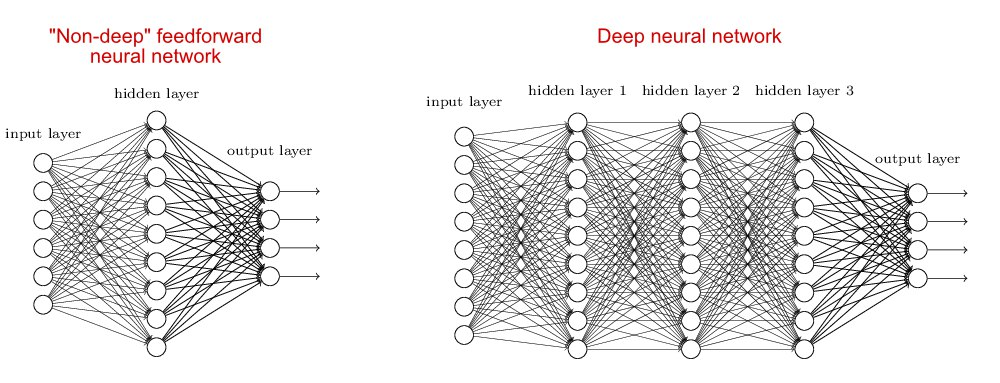
\includegraphics[scale=0.4]{figures/svsd.jpeg}
 %\end{wrapfigure}
\end{figure}

The main focus of~\cite{paper} and~\cite{gaia} is to demonstrate that
performance of the two kinds is comparable when using high level features
for the shallow one and low level features for the deep one. To achieve this
it is need a \textit{metric}, a measure of how well the classificator is
performing. Evaluating the metrics over the training, validation and test sets
is the primary technique for point out how the training process is going.
Therefore, is crucial to use the most significant ones.

The default metric provided by Keras~\cite{keras} is the binary accuracy.
Given an event if the output is greater than $0.5$ then it is classified
as signal, background otherwise. The right label is then compared and the
prediction correctness is determined. Done it for the entire considered
subset and found the right prediction percentage  the (binary) accuracy
is obtained.
Another metric widely used in Machine Learning is the result loss function
considered as a mean over a subset of events. This is the number that the
optimizer itself is trying to minimize so is a direct performing rate.
Despite this, it is significant in the training process only. It can not be
used in the final classifier rating not having a statistical meaning.
\begin{figure}[h]
 \centering
 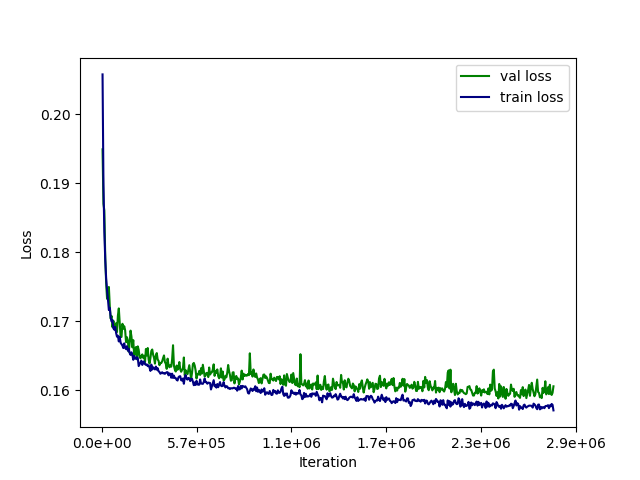
\includegraphics[scale=0.4]{figures/loss_tv.png}
 \caption{loss function during training}
\end{figure}

A more statistically significant approach is to find the \textit{AUC}
score, \ie~the \textit{Area Under the ROC Curve}, by drawing and
integrating the \textit{ROC Curve} that stands for \textit{Receiver
 Operating Characteristic}. Drawing the ROC curve is a graphical method to
observe binary classifiers efficiency. It is done by plotting percentage
successfully signal prediction (signal efficiency) versus the percentage
successfully background discovery \#(classification?) (background rejection).
The various points of the graph are obtained by varying the threshold in
the interval $\left[0,1\right]$ beyond which the Neural Network output it
considered signal, note that the binary accuracy is essentially the
ROC point which threshold is $0.5$.
\begin{figure}[h]
 \begin{minipage}{.5\textwidth}
  \centering
  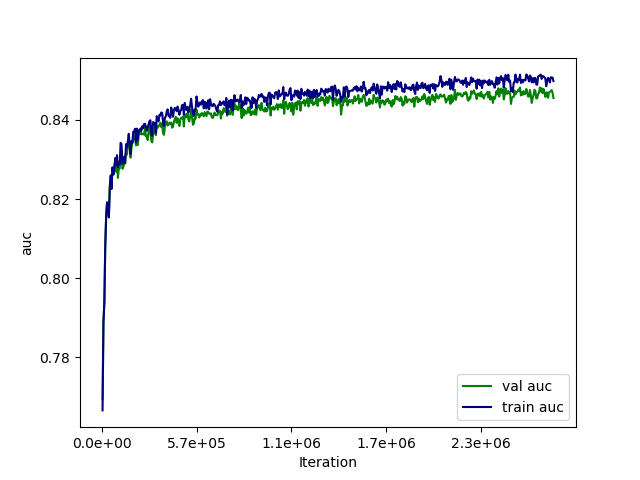
\includegraphics[scale=0.4]{figures/auc_tv.png}
  \caption{auc score during training}
 \end{minipage}\qquad%
 \begin{minipage}{.5\textwidth}
  \centering
  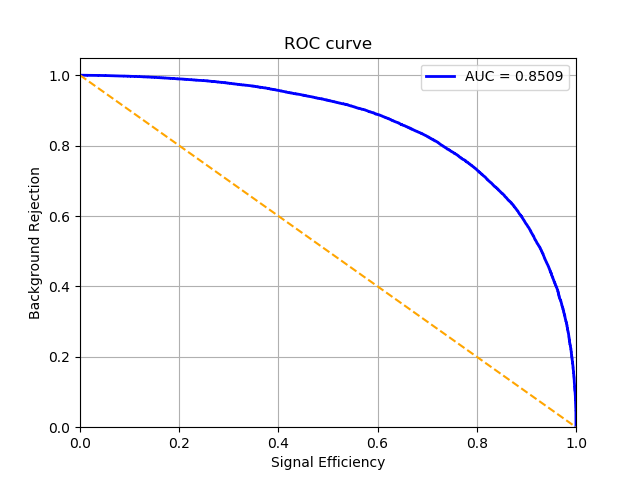
\includegraphics[scale=0.4]{figures/test_auc.png}
  \caption{test set auc score}
 \end{minipage}
\end{figure}

One more quantity that highlights the model behavior is called
\textit{Figure Of Merit} (\textit{FOM}). It is defined as
$FOM = \frac{S}{\sqrt{B}}$ where $S$ is the right classified signal events
total number and $B$ is right classified background events total number.
The term $\sqrt{B}$ represents the error on the number of background events
assuming they follow a Poisson distribution. More precisely, to state
whenever signal events $S$ are actually a resonance or only statistical
fluctuations, the effective error should take into account also the error on
the number of signal events, that is $\sqrt{S}$, as signal follow
poissonian distribution too. So the correct expression for the error would
be $\sigma = \sqrt{B + S}$. Nonetheless since $S \ll B$ the error can be
approximated as $\sigma \approx \sqrt{B}$.
\begin{figure}[h]
 \centering
 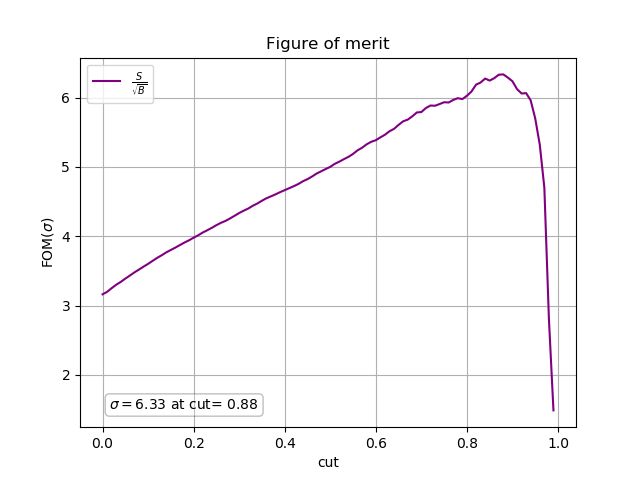
\includegraphics[scale=0.4]{figures/fom.png}
 \caption{Figure of merit of the test set}
\end{figure}

The data were simulated as described in Section~\ref{data} and they were
built such that signal and background would have the same probability.
The consequence is that the number of signals predicted events should be
quite the same of background predicted. In data collected by experiments, a
signal of new physics is usually a rare phenomenon which competes with
lots of standard processes included in background. Thus, the real cross
section of signal events may be so small that it may be confused with
background. $FOM$ computation allows finding the optimal cut point to
put in evidence the presence of signals. In fact, maximize this quantity
considered as a  function of the classifier acceptance threshold means
maximizing signal and background distribution over the phase space
expected by the theoretical model. A good cut point choice allows
physicists to determine whenever a difference in experimental
distributions can be identified as a new signal or not.

The last performance indicator that has been considered is the histogram
of the predicted events over the possible model outcomes. The network
discriminates well if the predicted signal distribution present a peak
towards $1$ and the predicted background distribution towards $0$.
\begin{figure}[h]
 \centering
 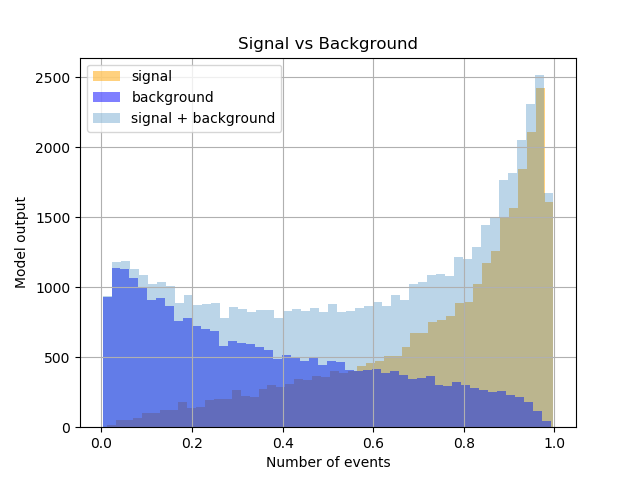
\includegraphics[scale=0.4]{figures/svb.png}
 \caption{Signal versus background in test set}
\end{figure}

\section{Shallow and deep Neural Networks performance}

In~\cite{gaia} some experiments have been done varying the number of layers,
neurons for layer and using various regularization techniques. The most
interesting result obtained is that the Deep Neural Networks trained and
tested with low level features perform the same (or better) than the Shallow
Neural Networks with high level features, which is excellent given the not
negligible work needed to develop high level features. The same results are
also found in~\cite{paper}.
\begin{figure}
 \centering
 \subfloat[][SN performance in~\cite{paper}]{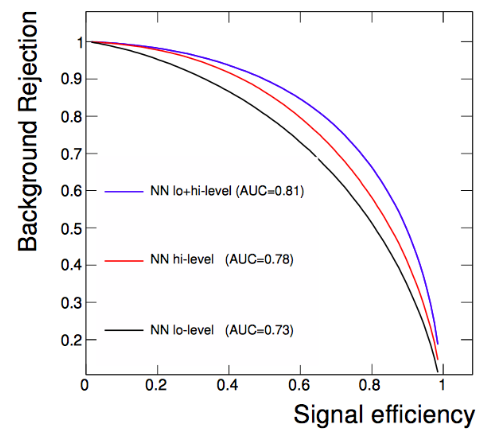
\includegraphics[width=.45\textwidth]{figures/SNp.png}} \quad
 \subfloat[][DN performance in~\cite{paper}]{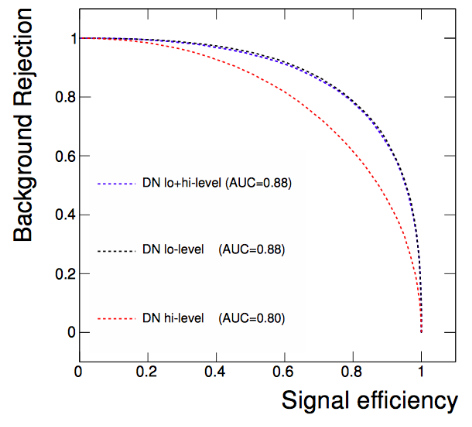
\includegraphics[width=.45\textwidth]{figures/DNp.png}} \\
 \subfloat[][SN performance in~\cite{gaia}]{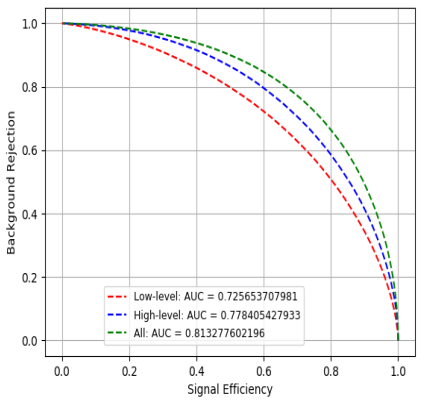
\includegraphics[width=.45\textwidth]{figures/SNg.png}} \quad
 \subfloat[][DN performance in~\cite{gaia}]{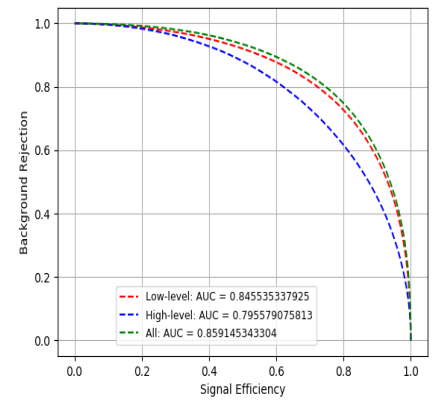
\includegraphics[width=.45\textwidth]{figures/DNg.png}} \\
 \caption{}
 \label{graphs}
\end{figure}
In Fig.~\ref{graphs} and in Tab.~\ref{table} are shown a comparison of the
performance with shallow neural networks (SNN) and deep neural networks
(DNN) in~\cite{paper} and~\cite{gaia} for three sets of input of features:
low level features, high level features and the complete set of features.
As can be seen, a shallow NN trained using only the low level features
performs significantly worse than one trained with only the high level
features. This is a well-known problem with shallow learning methods, and
motivates the calculation of high level features. Methods trained with only
the high level features, however, have a weaker performance than those
trained with the full set of features, which suggests that despite the
insight represented by the high level features, they do not capture all
the information contained in the low level features. The deep learning
techniques show close performance using the low level features
and the complete features, suggesting that they are automatically
discovering the insight contained in the high level features. The slightly
different performance in~\cite{paper} and~\cite{gaia} are explainable due
to the fact in~\cite{gaia} the algorithms can handle the training for
about $40$-$60$ epochs before overfitting, instead~\cite{paper} are able
to train for $200$-$1000$ which is a great difference. Even if the
quantitative results differ, the qualitative ones are the same.
\begin{table}
 \centering
 \subfloat[][AUC and discovery significance in~\cite{paper}]{
  \begin{tabular}{lccc}
   \toprule
   Technique                 & Low level   & High level  & Complete    \\
   \midrule
   $\text{SNN}_{\text{auc}}$ & $0.733$     & $0.777$     & $0.816$     \\
   $\text{DNN}_{\text{auc}}$ & $0.880$     & $0.800$     & $0.885$     \\
   $\text{SNN}_{\text{DS}}$  & $2.5\sigma$ & $3.1\sigma$ & $3.7\sigma$ \\
   $\text{DNN}_{\text{DS}}$  & $4.9\sigma$ & $3.6\sigma$ & $5.0\sigma$ \\
   \bottomrule
  \end{tabular}
 } \\
 \subfloat[][AUC and discovery significance in~\cite{gaia}]{
  \begin{tabular}{lccc}
   \toprule
   Technique                 & Low level    & High level   & Complete     \\
   \midrule
   $\text{SNN}_{\text{auc}}$ & $0.675$      & $0.763$      & $0.812$      \\
   $\text{DNN}_{\text{auc}}$ & $0.846$      & $0.796$      & $0.858$      \\
   $\text{SNN}_{\text{DS}}$  & $3.34\sigma$ & $3.69\sigma$ & $4.11\sigma$ \\
   $\text{DNN}_{\text{DS}}$  & $4.44\sigma$ & $3.85\sigma$ & $4.66\sigma$ \\
   \bottomrule
  \end{tabular}
 }
 \caption{}
 \label{table}
\end{table}

To understand if the obtained results can help to discriminate new signals
assumption was made that for $100$ signals events were $1000$ background
events as can be seen in Fig.\ref{res}. In order to simulate the physical
reality prediction histograms were re-normalized. The Tab.\ref{table} show
then that the discovery significance, which is a standard metric in
high-energy physics, can significantly improve even with small increases in
AUC.

\begin{figure}[hb]
 \centering
 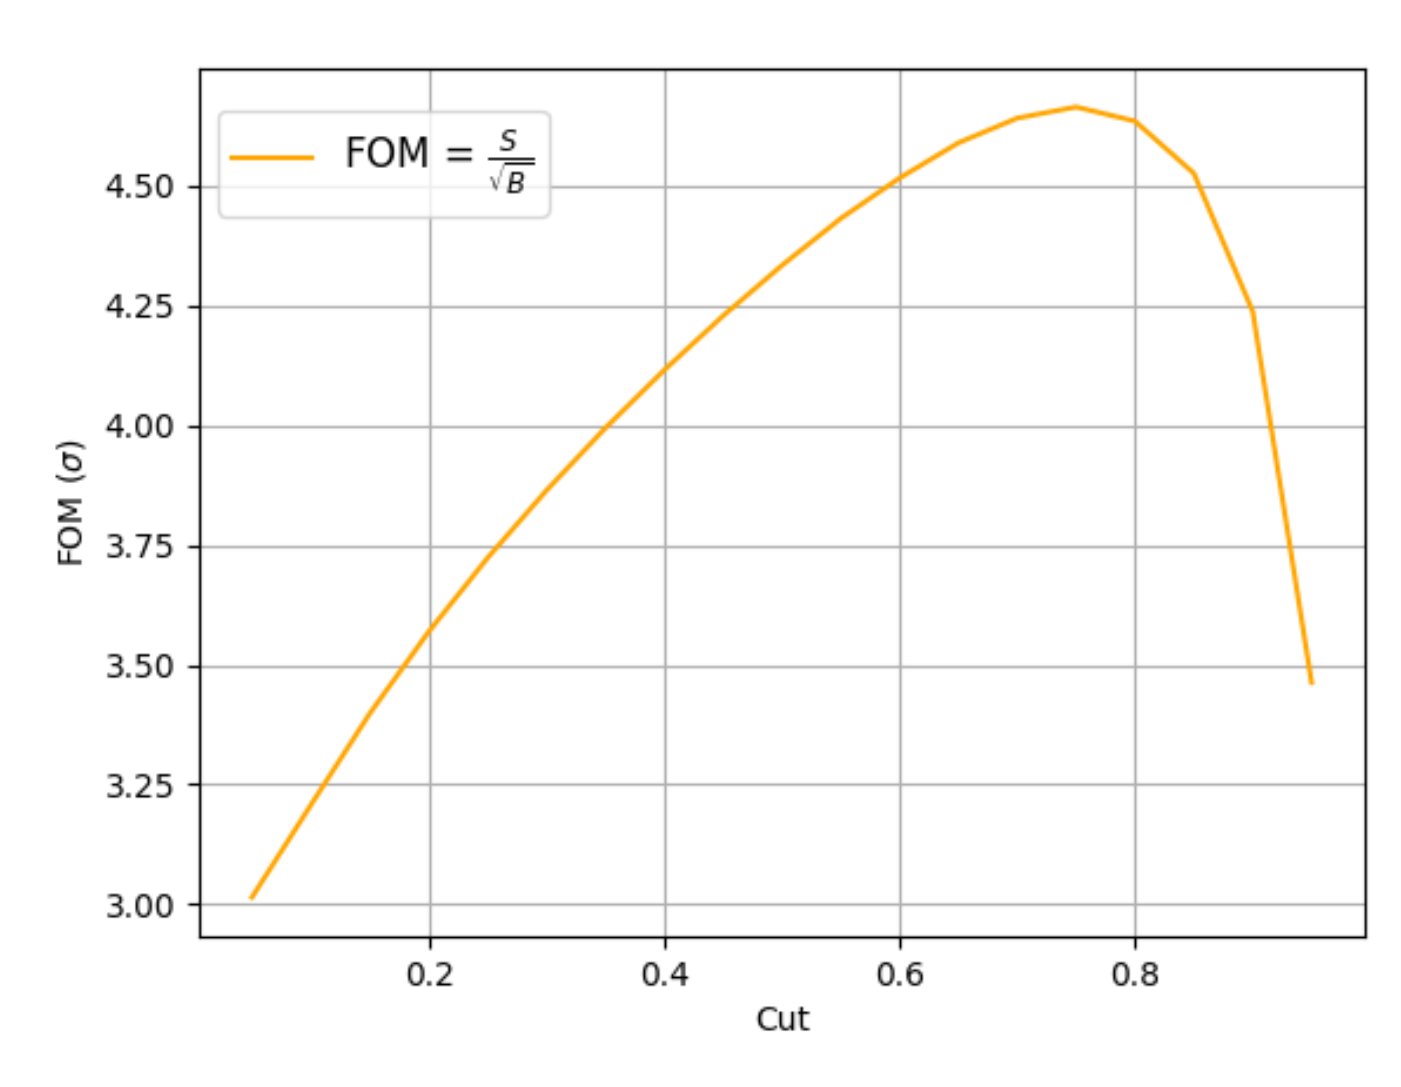
\includegraphics[width=.45\textwidth]{figures/fomr.png}
 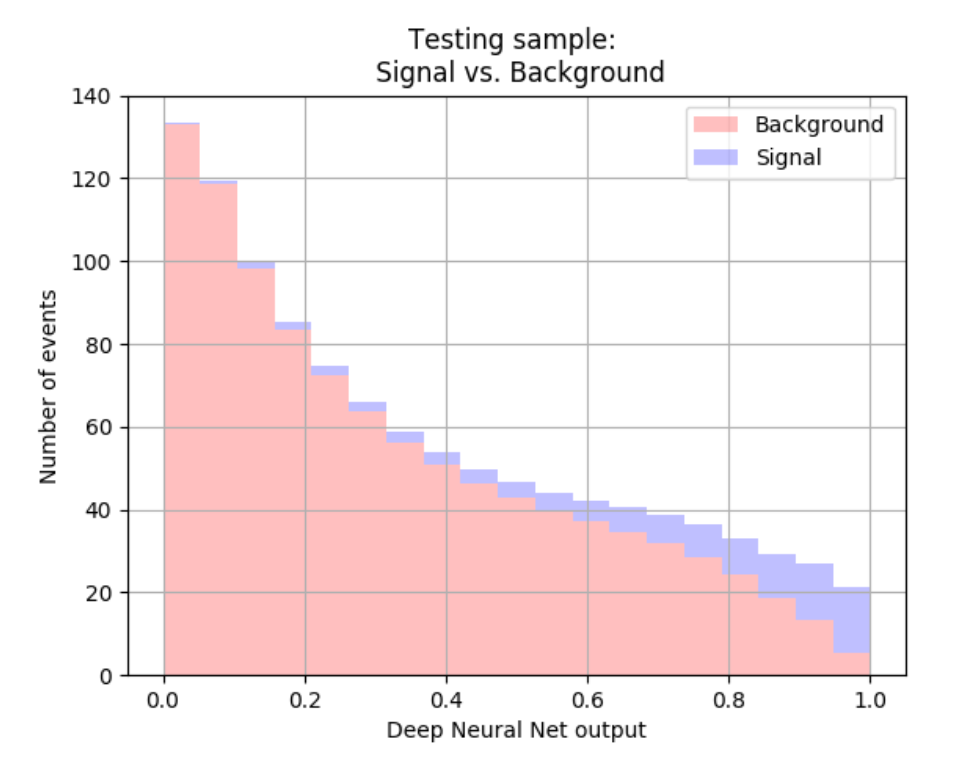
\includegraphics[width=.45\textwidth]{figures/svdbr.png}
 \caption{Figure of merit obtained after normalization in~\cite{gaia}}
 \label{res}
\end{figure}
